%\PassOptionToPackage{english}{babel}
\documentclass[french]{beamer}
\usetheme{Warsaw}
\usepackage{lmodern}
\usepackage[utf8]{inputenc}
\usepackage[T1]{fontenc}
\usepackage{babel}
\usepackage{color}
\usepackage{listings}
\usepackage{booktabs}
\usepackage{amsmath,amsthm,amssymb,graphicx,mathrsfs}
\usepackage{stmaryrd}
\usepackage{slashed}
%\usepackage[hmargin={3.5cm,3.5cm},top=4cm,bottom=4cm]{geometry} %problem...

\graphicspath{{images/}}

\newcommand{\vb}[1]{\mathbf{#1}}
\newcommand{\V}[1]{\textnormal{#1}}
\newcommand{\dd}[0]{\textrm{d}}
\newcommand{\bra}[1]{\langle#1 |}
\newcommand{\ket}[1]{| #1 \rangle}
\newcommand{\vdot}[0]{\boldsymbol\cdot}
\newcommand{\dom}{\mathrm{Dom}}

\newtheorem{remark}{Remark}
\newtheorem{proposition}{Proposition}

\setbeamertemplate{footline}[frame number]{}
%\setbeamertemplate{navigation symbols}{}
\setbeamertemplate{caption}[numbered]


%%%%%%%%%%%%%%%%%%%%%%%%%%%%
\lstset{%
  backgroundcolor=\color{white},   % choose the background color; you must add \usepackage{color} or \usepackage{xcolor}
  basicstyle=\small,        % the size of the fonts that are used for the code
  commentstyle=\color{blue},    % comment style
  extendedchars=true,              % lets you use non-ASCII characters; for 8-bits encodings only, does not work with UTF-8
  keepspaces=true,                 % keeps spaces in text, useful for keeping indentation of code (possibly needs columns=flexible)
  keywordstyle=\color{red},       % keyword style
  language=Fortran,                 % the language of the code
  rulecolor=\color{black},         % if not set, the frame-color may be changed on line-breaks within not-black text (e.g. comments (green here))
  showspaces=false,                % show spaces everywhere adding particular underscores; it overrides 'showstringspaces'
  showstringspaces=false,          % underline spaces within strings only
  showtabs=false,                  % show tabs within strings adding particular underscores
  stringstyle=\color{green},     % string literal style
  tabsize=2,                       % sets default tabsize to 2 spaces
  frame=single
}



%%%%%%%%%%%%%%%%%%%%%%%%%%%%%%%%%%%%%%%%%%%%%%%%%%%%%%%%%%%%%%%%%%%%%%%%
\title{Quantum field theories in external potentials}
\author{En-Hung CHAO}
\institute{Ecole Polytechnique}
\date{\today}
%%%%%%%%%%%%%%%%%%%%%%%%%%%%%%%%%%%%%%%%%%%%%%%%%%%%%%%%%%%%%%%%%%%%%%%%
%%%%%%%%%%%%%%%%%%%%%%%%%%%%%%%%%%%%%%%%%%%%%%%%%%%%%%%%%%%%%%%%%%%%%%%%
\begin{document}
%\selectlanguage{english}
%\graphicspath{{../images/}}

\begin{frame}
\titlepage%
\end{frame}
%%%%%%%%%%%%%%%%%%%%%%%%%%%%%%%%%%%%%%%
%%%%%%%%%%%%%%%%%%%%%%%%%%%%%%%%%
\begin{frame}
\frametitle{Outline}
\framesubtitle{}
\begin{enumerate}
 \item Introduction and motivation
%  \begin{enumerate}
%  \item Elements of Quantum Field Theory in Curved Space-Time (QFTCST)
%  \item Kondo effect
%  \item Brief review of AdS/CFT correspondence and holographic renormalization
%  \end{enumerate}
 \item Vacuum polarization in 1+1 dimension in presence of a Kondo type potential
%  \begin{enumerate}
%  \item Hadamard parametrix and vacuum polarization
%  \item Results
%  \end{enumerate}
 \item Wentzell boundary condition for Dirac fields
%  \begin{enumerate}
%  \item Well-posedness of an action
%  \item 3 examples
%  \item Vacuum polarization and stress-energy tensors in 1+1 dimension
%  \end{enumerate}
 \item Conclusion and prospective
\end{enumerate}
\end{frame}
%%%%%%%%%%%%%%%%%%%%%%%%%%%%%%%%%%%%%%%
\begin{frame}
\frametitle{Introduction}
\framesubtitle{Elements of QFTCST}

\color{blue}[S. Hollands, R.M. Wald Phys. Rep. 2015]

\begin{itemize}


\item Difficulty in defining the ground state in curved space-time for usual construction of Hilbert space
\item Algebraic approach formulated with an algebra of quantum observables $\mathscr{A}(M,g)$
\item Distributional nature of fields
\item Postulates for scalar field theory
 \begin{enumerate}
  \item \textbf{Linearity} $\phi(c_1 f_1 + c_2 f_2) = c_1 \phi(f_1) + c_2 \phi(f_2)$ for $c_1, c_2 \in \mathbb{C}$
%
\item \textbf{Klein-Gordon equation} $\phi\big( (\Box_g - m^2)f \big) = 0$
%
\item \textbf{Hermitian field} $\phi(f)^* = \phi(\bar{f})$
%
\item \textbf{Canonical commutation relation (CCR)} $[\phi(f_1), \phi(f_2)] = iE(f_1, f_2) \mathbf{1}$
 \end{enumerate}
\end{itemize}

\end{frame}
%%%%%%%%%%%%%%%%%%%%%%%%%%%%%%%%%%%%%%
\begin{frame}
\frametitle{Introduction}
\framesubtitle{Elements of QFTCST}
\begin{itemize}

\item \textbf{Physical state} $\omega: \mathscr{A}(M,g) \rightarrow \mathbb{C}$ with $\omega(\mathbf{1}) = 1$ and the positivity $\omega(a^*a) \geq 0$

\item \textbf{GNS construction} corresponding to the state 

\item \textbf{Hadamard states} propagation of the singularity of a Hadamard state in globally hyperbolic space-times
\\
\color{blue}[M.J. Radzikowski, Comm. Math. Phys.
, 179(3):529–553, 1996] \color{black}



\end{itemize}

\end{frame}
%%%%%%%%%%%%%%%%%%%%%%%%%%%%%%%%%%%%%%
\begin{frame}
\frametitle{Introduction}
\framesubtitle{Elements of QFTCST}

\begin{itemize}

\item Equivalent theory for Dirac field : Dirac equation and \textit{anti}-commutation relation
\\
\color{blue}[ H. Sahlmann and R. Verch
Rev. Math. Phys.
, 13:1203–
1246, 2001]\color{black}

\begin{equation*}
\{\psi(f_1), \psi(f_2)\} = i S(f_1, f_2) \mathbf{1}
\end{equation*}


\item \textbf{Hadamard states} and characterization
 \begin{equation*}
\begin{split}
\omega(\psi^B(x)\bar{\psi}_A(x')) + \omega(\bar{\psi}_A(x')\psi^B(x)) = &
iS^B_A(x,x') \\
\overline{\omega(\bar{\psi}(u)\psi(\bar{v}))} = & \omega(\bar{\psi}(v)\psi(\bar{u}))
\end{split}
\end{equation*}

\end{itemize}

\end{frame}
%%%%%%%%%%%%%%%%%%%%%%%%%%%%%%%%%%%%%%
\begin{frame}
\frametitle{Introduction}
\framesubtitle{Kondo effect}
\begin{itemize}
\item Anomalies in electrical resistance when temperature decreases

\begin{figure}[!h]
  \centering
  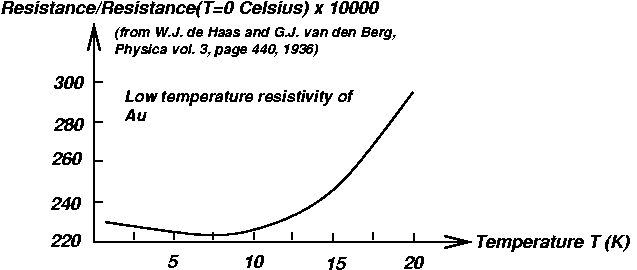
\includegraphics[height=0.4\textheight]{kondo}
\end{figure}

\end{itemize}

\end{frame}
%%%%%%%%%%%%%%%%%%%%%%%%%%%%%%%%%%%%%%
\begin{frame}
\frametitle{Introduction}
\framesubtitle{Kondo effect}
\begin{itemize}
\item Local spin interaction between electrons and impurities
\\
\color{blue}[J. Kondo
, 32(1):37, 1964]\color{black}

\item Hamiltonian
\\
\color{blue}[J. Erdmenger, C. Hoyos, A. O’Bannon and J. Wu, JHEP
, 12:086, 2013]\color{black}


\begin{equation*}
H = \psi_\alpha^\dagger \frac{-\nabla^2}{2m}\psi_\alpha +
\frac 1 2\lambda \delta(\vec{x})\vec{S}\cdot \psi_{\alpha'}^\dagger  \vec{\sigma}_{\alpha' \alpha} \psi_\alpha
\end{equation*}

\item How could such a local interaction change the vacuum polarization ?
\end{itemize}

\end{frame}
%%%%%%%%%%%%%%%%%%%%%%%%%%%%%%%%%%%%%%
\begin{frame}
\frametitle{Introduction}
\framesubtitle{Holographic renormalization}

\begin{itemize}
\item Strong/weak coupling duality and IR-UV connection in anti-deSitter/Conformal Field Theory (AdS/CFT) correspondence

\item Example for scalar field

\begin{equation*}
\begin{split}
\mathcal{S}[\phi] = & -\int_{B_{d+1}} \sqrt{g} \phi D_i D^i \phi + 
\lim_{\epsilon\rightarrow 0}\int_{T_\epsilon}  \sqrt{h} \phi (\vec{n}\cdot\vec{\nabla})\phi \\
%
& \sim \int \dd \mathbf{x} \dd \mathbf{x}' 
\frac{\phi_0(\mathbf{x})\phi_0(\mathbf{x}')}{|\mathbf{x} - \mathbf{x}'|^{2d}}
\end{split}
\end{equation*}

$\Rightarrow$ the same divergence as in CFT

\end{itemize}

\end{frame}
%%%%%%%%%%%%%%%%%%%%%%%%%%%%%%%%%%%%%%
\begin{frame}
\frametitle{Introduction}
\framesubtitle{Holographic renormalization}

\begin{itemize}

\item Boundary field and holographic renormalization
\\
\color{blue}[K. Skenderis
Class. Quant. Grav.
,
19:5849–5876, 2002]\color{black}

\item Type of action appearing in holographic renormalization for scalar case
\begin{equation*}
\begin{split}
\mathcal{S} = & \mathcal{S}_{\mathrm{bulk}} + \mathcal{S}_{\mathrm{bdy}}
\\ = &
-\frac 1 2 \int_M g^{\mu\nu} \partial_\mu \phi \partial_{\nu} + 
\mu^2\phi^2 - \frac c 2 \int_{\partial M}h^{\mu\nu}\partial_\mu\phi\partial_\nu\phi + \mu^2\phi^2
\end{split}
\end{equation*}

\color{blue}[J. Zahn,  arXiv:1512.05512v2]\color{black}

\item The case of Dirac fields and the vacuum polarization under the new boundary condition (generalized bag boundary condition)?

\end{itemize}

\end{frame}
%%%%%%%%%%%%%%%%%%%%%%%%%%%%%%%%%%%%%%
\begin{frame}[shrink=20]
\frametitle{Vacuum polarization in 1+1 dimension in presence of a Kondo type potential}
\framesubtitle{Hadamard parametrix and vacuum polarization}

\begin{itemize}
\item Representation of the Dirac gamma matrices
\begin{equation*}
\gamma^0 = \begin{pmatrix}
0 & 1 \\
1 & 0 \end{pmatrix}  \quad  \gamma^1 = \begin{pmatrix}
0  & 1 \\
-1 & 0
\end{pmatrix}
\end{equation*}

\item Hadamard parametrix for a spin-$\frac 1 2$ massless particle with charge $+e$ with external potential $A^\mu(x) = (Ex^1, 0 )$

\color{blue}[J. Schlemmer and J. Zahn, Ann. of Phys. 2015]\color{black}

\begin{equation*}
\begin{split}
& H^\pm (x, y)^1_2 = \frac{-i}{2\pi}\frac{1-\frac i 2 e E(x^1 + y^1)(x^0-y^0) 
- \frac 1 8 (eE)^2(x^1 + y^1)^2(x^0 - y^0)^2}{x^0 - y^0 + x^1 - y^1 \mp i \epsilon}  \\
& H^\pm (x, y)^2_1 = \frac{-i}{2\pi}\frac{1-\frac i 2 e E(x^1 + y^1)(x^0-y^0) 
- \frac 1 8 (eE)^2(x^1 + y^1)^2(x^0 - y^0)^2}{x^0 - y^0 - x^1 + y^1 \mp i \epsilon}
\end{split}
\end{equation*}

\end{itemize}

\end{frame}
%%%%%%%%%%%%%%%%%%%%%%%%%%%%%%%%%%%%%%
\begin{frame}
\frametitle{Vacuum polarization in 1+1 dimension in presence of a Kondo type potential}
\framesubtitle{Hadamard parametrix and vacuum polarization}

 Dirac's method and vacuum current as a Hadamard state

\begin{equation*}
\begin{split}
\omega(\psi^B(x)\bar{\psi}_A(y)) = & \int_{E_k >0} \psi_k^B(x)\bar{\psi}_{A,k}(y)e^{-i(x^0-y^0)E_k} \dd k \\
\omega(\bar{\psi}_A(y)\psi^B(x)) = & \int_{E_k <0} \psi_k^B(x)\bar{\psi}_{A,k}(y)e^{-i(x^0-y^0)E_k} \dd k 
\end{split}
\end{equation*}

\begin{equation*}
j^\mu(x) = \lim_{y \rightarrow x} \gamma^A_B \big(
\omega(\psi^B(x)\bar{\psi}_A(y)) - H^B_A (x, y)\big)
\end{equation*}

\end{frame}
%%%%%%%%%%%%%%%%%%%%%%%%%%%%%%%%%%%%%%
\begin{frame}
\frametitle{Vacuum polarization in 1+1 dimension in presence of a Kondo type potential}
\framesubtitle{Hadamard parametrix and vacuum polarization}

\begin{equation*}
\begin{split}
& T_{00} = \frac{i}{2} (\bar{\psi} \gamma_1 \nabla_1 \psi - \nabla_1 \bar{\psi}\gamma_1 \psi)  \\
& T_{11} = \frac{i}{2} (\bar{\psi} \gamma_0 \nabla_0 \psi - \nabla_0 \bar{\psi}\gamma_0 \psi)  \\
& T_{01} = \frac{i}{4} (\bar{\psi} \gamma_1 \nabla_0 \psi +\bar{\psi} \gamma_0 \nabla_1 \psi - \nabla_1 \bar{\psi}\gamma_0 \psi - \nabla_0 \bar{\psi}\gamma_1 \psi)  
\end{split}
\end{equation*}

Renormalization of the stress-energy tensor

\begin{equation*}
\begin{split}
T_{00}(x,y) = 
\frac{i}{2}\Big( & 
\nabla_{x^1}\big(\omega(  \psi^B(x) \bar{\psi}_A(y))-H^B_A(x,y)\big)(\gamma_1)^A_B \\
& - \nabla_{y^1}\Big(\omega( \psi^B(x)  \bar{\psi}_A(y)) - H^B_A(x,y)\big)(\gamma_1)^A_B \Big)   
\end{split}
\end{equation*}


\end{frame}
%%%%%%%%%%%%%%%%%%%%%%%%%%%%%%%%%%%%%%
\begin{frame}[shrink=10]
\frametitle{Vacuum polarization in 1+1 dimension in presence of a Kondo type potential}
\framesubtitle{Results}

We start with $E = 0$ and a confined space $x^1 \in [\-\frac L 2 , \frac L 2]$
\begin{itemize}
\item We denote $\phi = \gamma^0\psi$ where $\psi$ is a massless Dirac field satisfying 
\begin{equation*}
i\gamma^\mu\partial_\mu \psi = 0
\end{equation*}
outside the singularity
\item Imposing a Kondo type potential due to the impurity at $x^1 = 0$,
we consider $\phi$ satisfying

\begin{equation*}
i \partial_0 \phi = 
\begin{pmatrix} 
-1 & 0 \\
0 & 1 
\end{pmatrix} i \partial_1 \phi +
\begin{pmatrix}
v_3 & v_- \\
v_+ & -v_3
\end{pmatrix} \delta(x_1) \phi
\end{equation*}
where $v_3, v_+ + v_- \in \mathbb{R}$ and $ v_+ - v_-\in i \mathbb{R}$
\end{itemize}

\end{frame}
%%%%%%%%%%%%%%%%%%%%%%%%%%%%%%%%%%%%%%
\begin{frame}
\frametitle{Vacuum polarization in 1+1 dimension in presence of a Kondo type potential}
\framesubtitle{Results}

\begin{itemize}
\item Matching condition at $x^1 = 0$ for $\phi =
\begin{pmatrix}
\phi_L \\
\phi_R
\end{pmatrix}$

\begin{equation*}
\begin{pmatrix}
\phi_L(0^+) \\
\phi_R(0^+)
\end{pmatrix} = \begin{pmatrix}
\frac{A}{D}  & \frac{C}{D} \\
\frac{C^*}{D} & \frac{A}{D}
\end{pmatrix}\begin{pmatrix}
\phi_L(0^-) \\
\phi_R(0^-)
\end{pmatrix}
\end{equation*}
where  $\Sigma = v_+ ^ 2 + v_- ^ 2 + v_3 ^ 2$, $A = 1+ \frac{1}{4}\Sigma$, $C = -iv_-$, $D = 1-\frac{1}{4}\Sigma + iv_3$.

\item Bag boundary condition (in terms of $\psi = \gamma^0\phi$)
\begin{equation*}
i\gamma^1 \psi \Big\vert_{\pm \frac{L}{2}} = \pm \psi \Big\vert_{\pm \frac{L}{2}}
\end{equation*}

\item The problem is well posed because the Hamiltonian of the dynamical system is self-adjoint under these conditions

\end{itemize}

\end{frame}
%%%%%%%%%%%%%%%%%%%%%%%%%%%%%%%%%%%%%%
\begin{frame}[shrink=10]
\frametitle{Vacuum polarization in 1+1 dimension in presence of a Kondo type potential}
\framesubtitle{Results}

We denote $\eta = \arg C$

\begin{itemize}

\item Mode expansion
\begin{equation*}
\begin{split}
k_{n} = \frac{1}{L} \big(\theta + (\pi - \theta)(1- (-1)^n)\big) + \frac{\pi}{L}n \\
\quad \textrm{where $\theta = \arccos\bigg( \frac{-|C| \sin \eta}{A} \bigg)$}
\end{split}
\end{equation*}


\item Solutions
\begin{equation*}
\begin{split}
\phi_{k_{n}} = 
& \sqrt{\frac{1}{L(\alpha - \beta \sin (k_{n}L - \eta))}} \Bigg( 
\begin{pmatrix}
1 & 0 \\
0  & e^{-i(kL + \frac{\pi}{2})}
\end{pmatrix}
\Theta(-x^1) + \\
& \begin{pmatrix}
\frac{A}{D}  +  \frac{C}{D} e^{-i(kL + \frac{\pi}{2})} & 0 \\
0  & \frac{C^*}{D}  + \frac{A}{D}e^{-i(kL + \frac{\pi}{2})}
\end{pmatrix}\Theta(x^1)\Bigg)
\begin{pmatrix}
e^{ik_{n} x^1} \\
e^{- ik_{n} x^1}
\end{pmatrix}
\end{split}
\end{equation*}


\end{itemize}

\end{frame}
%%%%%%%%%%%%%%%%%%%%%%%%%%%%%%%%%%%%%%
\begin{frame}
\frametitle{Vacuum polarization in 1+1 dimension in presence of a Kondo type potential}
\framesubtitle{Results}

\begin{itemize}

\item Charge density

\begin{equation*}
\begin{split}
\rho(x) = \frac{e}{\pi L}\Big( \frac{\beta \sin \theta \cos \eta}{\alpha + \beta \sin \eta \cos \theta}\Big) (-\theta + \pi) \Big( \Theta(-x^1) - \Theta(x^1)\Big)
\end{split}
\end{equation*}
and the current density is zero. 

\item Stress-energy tensor
\begin{equation*}
T_{\mu\nu} = \frac{ \pi}{2 L^2} \big( -\frac{1}{3} + \frac{(\theta - \pi)^2}{\pi^2}\big)\begin{pmatrix}
1  & 0 \\ 0  &  1
\end{pmatrix}
\end{equation*}
\end{itemize}

\end{frame}
%%%%%%%%%%%%%%%%%%%%%%%%%%%%%%%%%%%%%%
\begin{frame}[shrink=5]
\frametitle{Vacuum polarization in 1+1 dimension in presence of a Kondo type potential}
\framesubtitle{Results}

Other cases
\begin{itemize}
\item Confined space with potential $(A_0, A_1) = (Ex^1, 0)$
\begin{equation*}
\rho(x) = \frac{e}{\pi L}\Big( \frac{\beta \sin \theta \cos \eta}{\alpha + \beta \sin \eta \cos \theta}\Big) (-\theta + \pi)
\Big(\Theta(- x^1) - \Theta(x^1))\Big) + \frac{e^2 E}{\pi} x^1
\end{equation*}
\begin{equation*}
T_{ab}(x) = 
\bigg( \frac{\pi}{2L^2}\big( -\frac{1}{3} + \frac{(\theta - \pi)^2}{\pi^2}\big) + \frac{e^2E^2(x^1)^2}{2 \pi} \bigg)
\begin{pmatrix}
1 & 0 \\ 0 & 1
\end{pmatrix}
\end{equation*}

\item Unconfined space : the punctual interaction potential has no influence

\end{itemize}

$\Longrightarrow$ The presence of the Kondo potential opposite offsets in the two regions separated by the singularity. 

\end{frame}
%%%%%%%%%%%%%%%%%%%%%%%%%%%%%%%%%%%%%%
\begin{frame}[shrink=5]
\frametitle{Wentzell boundary condition for Dirac fields}
\framesubtitle{Well-posedness of an action}

$\mathcal{M}$ a d+1 dimensional spin manifold (Minkowski) with time-like static boundary $\partial\mathcal{M}$
\begin{itemize}
\item We propose to study the following action
\begin{equation*}
\mathcal{S} = \frac{1}{2}i\int_{\mathcal{M}} \bar{\psi} \gamma^\mu \partial_\mu \psi - \partial_\mu \bar{\psi} \gamma^\mu \psi 
+ \frac{1}{2}\int_{\partial \mathcal{M}} ic \bar{\psi} \gamma^\alpha \partial_\alpha (1 - i \gamma^\bot) \psi
+ \bar{\psi} \psi
\end{equation*}

\item Equation of motion in terms of $\phi = \gamma^0 \psi$
\begin{equation*}
\begin{cases}
i \partial_0 \phi = i \gamma^0 \gamma^j \partial_j \phi   \quad \textrm{in $\mathcal{M}$}\\
i \partial_0(1 + i\gamma^\bot) \phi = i\gamma^0 \gamma^a \partial_a (1+ i\gamma^\bot)\phi - c^{-1} \gamma^0(1 - i \gamma^{\bot})\phi \quad \textrm{on $\partial \mathcal{M}$}
\end{cases}
\end{equation*}

\end{itemize}

\end{frame}
%%%%%%%%%%%%%%%%%%%%%%%%%%%%%%%%%%%%%%
\begin{frame}
\frametitle{Wentzell boundary condition for Dirac fields}
\framesubtitle{Well-posedness of an action}
The Hamiltonian of the problem

\begin{equation*}
\Delta = \begin{pmatrix}
i \gamma^0 \slashed{\partial}  & 0 \\
-c^{-1} \gamma^0 \mathcal{P}_- \cdot \vert_{\partial M}&  i\gamma^0 \slashed{\partial}_| \mathcal{P}_+
\end{pmatrix}
\end{equation*}
where $\slashed{\partial} = \gamma^j\partial_j$ for
$j \in \llbracket 1 , d \rrbracket$ and $\slashed{\partial}_| = h^{ab} \gamma_{a} \partial_{a}$ where $h$ is the second fundamental form.

$\mathcal{P}_+$ is the projector defined by
\begin{equation*}
\mathcal{P}_\pm = \frac{1}{2}(1 \pm i n_j\gamma^j) 
\end{equation*}

\end{frame}
%%%%%%%%%%%%%%%%%%%%%%%%%%%%%%%%%%%%%%
\begin{frame}[shrink=10]
\frametitle{Wentzell boundary condition for Dirac fields}
\framesubtitle{Well-posedness of an action}

\begin{itemize}

\item Hilbert space $\mathcal{H} = L^{2}(M)\times L^{2}(\partial M, \mathcal{P}_+ F)$
where $M$ is an equal-time hypersurface of $\mathcal{M}$ and $\partial M = M\cap \partial \mathcal{M}$ with inner product
\begin{equation*}
\langle \cdot, \cdot \rangle _\mathcal{H} = \langle \cdot, \cdot \rangle _{L^2(M)} + c \langle \cdot, \cdot \rangle _{L^2(\partial M)}
\end{equation*}

\item $\Delta$ is self-adjoint on 

\begin{equation*}
\dom( \Delta) = \{ \Phi = (\phi, \phi_|) \in W^{1,2}(M)\times W^{1,2}(
\partial M) \enskip | \enskip \mathcal{P}_+\phi \vert_{\partial M} - \phi_| = 0 \} 
\end{equation*}  

\end{itemize}

\end{frame}
%%%%%%%%%%%%%%%%%%%%%%%%%%%%%%%%%%%%%%
\begin{frame}[shrink=10]
\frametitle{Wentzell boundary condition for Dirac fields}
\framesubtitle{Well-posedness of an action}

We denote 
\begin{equation*}
\mathcal{H}^k(M) = \cap_{s=0}^{k} \dom(\Delta), 
\quad
\| \cdot \|_{\mathcal{H}^k(M)} = \| \Delta^k \cdot \|_{\mathcal{H}(M)}
\end{equation*}

\begin{equation*}
\mathcal{H}_\varepsilon^k(M) \equiv
\{ \Phi \in \mathcal{H}^k(M) \enskip\big\vert\enskip \| \Delta^k \Phi\| \geq \varepsilon \| \Phi\| \}
\end{equation*}

%\begin{equation*}
%\Phi_0\in \cap_{k\in\mathbb{N}}\overline{\mathcal{H}^k_{\varepsilon_k}(M) }
%\end{equation*}

\begin{proposition}
Let $\Sigma_0$ and $\Sigma_1$ two equal-time surfaces.
Let $k \in \mathbb{N}^*$.
Suppose that the initial data $\Phi_0 = (\phi, \phi_|)\in \cap_{k\in\mathbb{N}}\overline{\mathcal{H}^k_{\varepsilon_k}(M) }$.
%With the same notations and the same conditions as in \cref{wen-propcau}, 
The smooth solution $\Phi$ depends continuously on the initial data $(\phi, \phi_|)$ on a Cauchy surface $\mathcal{S}_0 \subset \Sigma_0$ in the sense that
\begin{equation*}
\big\| \frac{\partial^k}{\partial t^k} \Phi\big\|_{\mathcal{H}(\mathcal{S}_1)}
\leq
\big\| \Phi\big\|_{\mathcal{H}^{k}(\mathcal{S}_0)}
\end{equation*}
for any $\mathcal{S}_1 \in D^+(\mathcal{S}_0)\cap\Sigma_1$
where $D^+(\mathcal{S}_0)$ is the future domain of dependence of $\mathcal{S}_0$.
\end{proposition}

\end{frame}
%%%%%%%%%%%%%%%%%%%%%%%%%%%%%%%%%%%%%%
\begin{frame}[shrink=20]
\frametitle{Wentzell boundary condition for Dirac fields}
\framesubtitle{Well-posedness of an action}
\textbf{Sketch of the proof}

\begin{enumerate}
\item 
\begin{equation*}
\begin{split}
\big\| \frac{\partial }{\partial t} \Phi \big\|^2_\mathcal{H}   = &
\langle \Phi, \Delta^2 \Phi \rangle_{\mathcal{H}} = 
\|\nabla \phi \|^2_{L^2 (M)} + c^{-1} \| \mathcal{P}_- \phi\vert_{\partial M} \|^2_{L^2(\partial M)}
+ c \| \mathcal{P}_+ \nabla \phi\vert_{\partial M} \|^2_{L^2(\partial M)}
\end{split}
\end{equation*}
where $\nabla$ is the gradient.

\item We introduce 
\begin{equation*}
\begin{split}
& T_{\mu\nu} = \partial_{(\mu} \phi^\dagger \partial_{\nu)} \phi - \frac{1}{2}g_{\mu\nu} \partial_\lambda\phi^\dagger\partial^\lambda\phi  \\
& T_{|\alpha\beta} = c\Big( \partial_{(\alpha}\mathcal{P}_+\phi^\dagger_| \partial_{\beta)}\mathcal{P}_+\phi_| - 
\frac{1}{2}h_{\alpha\beta}\big( \partial_\gamma\mathcal{P}_+\phi^\dagger_| \partial^\gamma\mathcal{P}_+\phi_|
 - c^{-2}|\mathcal{P}_- \phi\vert_{\partial M}|^2 \big)\Big) 
\end{split}
\end{equation*}
which satisfy the dominant energy condition
\begin{equation*}
\begin{split}
T_{\mu\nu} \xi^\mu \xi^\nu \geq 0 \quad \mathrm{ and }\quad
T_{\alpha\beta} \xi^\alpha \xi^\beta \geq 0 
\quad\textrm{ for $\xi$ time-like}
\end{split}
\end{equation*}

\item Integrate $\partial^\mu T_{\mu\nu}\xi^\nu = 0$ with $\xi$ future directed on a well-chosen domain.

\end{enumerate}

\end{frame}
%%%%%%%%%%%%%%%%%%%%%%%%%%%%%%%%%%%%%%
\begin{frame}
\frametitle{Wentzell boundary condition for Dirac fields}
\framesubtitle{Vacuum polarization and stress-energy tensors in 1+1 dimension}

\begin{itemize}

\item Spatially confined in $x^1 \in [-L, L]$
\begin{equation*}
\gamma^0 = \begin{pmatrix} 0 & 1 \\ 1 & 0 \end{pmatrix} \quad
\gamma^1 = \begin{pmatrix} 0 & -1 \\ 1 & 0 \end{pmatrix}
\quad
 \mathcal{P}_\pm = \frac 1 2  \begin{pmatrix} 1 & \mp i \\ \pm i & 1 \end{pmatrix}
\end{equation*}

\item Let $\Phi = (\phi, \phi_|)$ where $\phi = \begin{pmatrix} \phi_L \\ \phi_R \end{pmatrix}$ \\
Well-posedness $\Longrightarrow$
\begin{equation*}
\phi_L = \sum f_n e^{-ik_n(x^0 - x^1)} \quad
\phi_R = \sum g_n e^{-ik_n(x^0 + x^1)}
\end{equation*}
\end{itemize}
\end{frame}
%%%%%%%%%%%%%%%%%%%%%%%%%%%%%%%%%%%%%%
\begin{frame}
\frametitle{Wentzell boundary condition for Dirac fields}
\framesubtitle{Vacuum polarization and stress-energy tensors in 1+1 dimension}

\begin{itemize}
\item Asymptotic behavior of the modes and the normalization constants

\begin{equation*}
k_n = \frac 1 L \Big( \big( \frac n 2 + \frac 1 4 \big)\pi + \frac{2}{\pi C n}+ \mathcal{O}\big(\frac{1}{n^3}\big) \Big)
\end{equation*}

\begin{equation*}
|f_n|^2 = |g|^2=
\frac{1}{4L}\Big( 1 - \frac{4}{\pi^2C n^2} + \mathcal{O}\big(\frac{1}{n^3}\big) \Big)
\end{equation*}

\item Renormalized vacuum current and stress-energy tensor

\begin{equation*}
\rho = e \sum_{n=0}^{+\infty}\big(|f_n|^2 -\frac{1}{4L} \big)
\end{equation*}


\end{itemize}
\end{frame}
%%%%%%%%%%%%%%%%%%%%%%%%%%%%%%%%%%%%%%
\begin{frame}
\frametitle{Conclusion and prospective}



\begin{itemize}

\item To summerize
 \begin{itemize}
 \item The offset effect of Kondo type potential on vacuum polarization using Dirac's prescription
 \item Alternative and generalization of the bag boundary condition
 \item Effect of the boundary field on vacuum polarization 
 \end{itemize}

\item Prospective
 \begin{itemize}
 \item Generalization of boundary conditions of vector fields and gauge fields
 \item Causal propagation of the 0 modes
 \item Application in holographic renormalization
 \end{itemize}

\end{itemize}


\end{frame}
%%%%%%%%%%%%%%%%%%%%%%%%%%%%%%%%%%%%%%
\begin{frame}
\frametitle{Wentzell boundary condition for Dirac fields}
\framesubtitle{Vacuum polarization and stress-energy tensors in 1+1 dimension}



\end{frame}
%%%%%%%%%%%%%%%%%%%%%%%%%%%%%%%%%%%%%%
\begin{frame}
\frametitle{Wentzell boundary condition for Dirac fields}
\framesubtitle{2 examples}

\begin{proposition}
Let $M = \mathbb{R}^{d-1} \times \mathbb{R}_+$. $\Delta$ is a self-adjoint operator with spectrum $\mathbb{R}$
\end{proposition}

\textit{remark}
The causal propagation can not be guaranteed by the previous proof due to the existence of the 0 modes.


\end{frame}
%%%%%%%%%%%%%%%%%%%%%%%%%%%%%%%%%%%%%%

\begin{frame}
\frametitle{Wentzell boundary condition for Dirac fields}
\framesubtitle{2 examples}

\begin{proposition}
Let ${M} = \mathbb{R}^{d-1} \times [-L, L]$.
In the case where $\cos c^{-1}L \neq 0$,
the spectrum is discrete.
For any mode $k$, there exists $p_d\in \mathbb{R}$ 
satisfying 

\begin{equation*}
\tan p_d L = \frac{p_d \pm c^{-1}}{p_d \mp c^{-1}}
\end{equation*}

and $-p^jp_j = k^2$.
\end{proposition}


\end{frame}
%%%%%%%%%%%%%%%%%%%%%%%%%%%%%%%%%%%%%%

\end{document}
















